\documentclass[12pt]{article}
\usepackage[ddmmyyyy]{datetime} 
\usepackage[margin=1in]{geometry}
\usepackage{amsmath,amssymb,amsfonts} % Gộp chung các package toán
\usepackage{fancyhdr}
\usepackage{graphicx}
\usepackage{float}
\usepackage{cancel}
\usepackage{subcaption}
\usepackage[utf8]{vietnam}
\usepackage{makecell}
\usepackage{blindtext}
\usepackage{xcolor}
\usepackage{enumitem}
\usepackage{listings}
\usepackage{algorithm}
\usepackage{algpseudocode}
\usepackage{longfbox} 
\usepackage{hyperref}
\usepackage{booktabs}
\usepackage{tabularx}
\usepackage{tcolorbox}
\usepackage{colortbl}
\usepackage{multicol}
\usepackage{lipsum}

% Fix lỗi biblatex: Chỉ khai báo 1 lần duy nhất ở đây
% Nếu bạn muốn dùng style khác (như apa, ieee), hãy sửa ở phần style
\usepackage[style=numeric,backend=biber]{biblatex}

\setlength{\headheight}{30pt}

% Định nghĩa màu sắc cho Code
\definecolor{codegreen}{rgb}{0,0.6,0}
\definecolor{codegray}{rgb}{0.5,0.5,0.5}
\definecolor{codepurple}{rgb}{0.58,0,0.82}
\definecolor{backcolour}{rgb}{0.95,0.95,0.92}
\definecolor{cpptype}{rgb}{0.16, 0.47, 0.68}     % Màu xanh cho kiểu dữ liệu
\definecolor{cppfunc}{rgb}{0.6, 0.3, 0.1}        % Màu nâu/cam cho tên hàm
\definecolor{cppvar}{rgb}{0.1, 0.5, 0.5}         % Màu teal cho tên biến


% Định nghĩa Style chung
\lstdefinestyle{mystyle}{
    backgroundcolor=\color{backcolour},   
    commentstyle=\color{codegreen},
    keywordstyle=\color{magenta},
    numberstyle=\tiny\color{codegray},
    stringstyle=\color{codepurple},
    basicstyle=\ttfamily\footnotesize,
    breakatwhitespace=false,         
    breaklines=true,                 
    captionpos=b,                    
    keepspaces=true,                 
    numbers=left,                    
    numbersep=5pt,                  
    showspaces=false,                
    showstringspaces=false,
    showtabs=false,                  
    tabsize=2,
    inputencoding=utf8, % Đổi utf8x thành utf8 để ổn định hơn
    extendedchars=true,
    % Thêm ký tự đặc biệt ± để tránh lỗi compile
    literate=%
    {±}{{$\pm$}}1
    % Vần tiếng Việt (Giữ nguyên phần literate của bạn ở đây)
    {á}{{\'a}}1 {à}{{\`a}}1 {ạ}{{\d a}}1 {ả}{{\h a}}1 {ã}{{\~ a}}1
    {Á}{{\'A}}1 {À}{{\`A}}1 {Ạ}{{\d A}}1 {Ả}{{\h A}}1 {Ã}{{\~ A}}1
    {ă}{{\u a}}1 {ắ}{{\'\abreve }}1 {ằ}{{\`\abreve }}1 {ặ}{{\d \abreve }}1 {ẳ}{{\h \abreve }}1 {ẵ}{{\~\abreve }}1
    {Ă}{{\u A}}1 {Ắ}{{\'\ABREVE }}1 {Ằ}{{\`\ABREVE }}1 {Ặ}{{\d \ABREVE }}1 {Ẳ}{{\h \ABREVE }}1 {Ẵ}{{\~\ABREVE }}1
    {â}{{\^ a}}1 {ấ}{{\'\acircumflex }}1 {ầ}{{\`\acircumflex }}1 {ậ}{{\d \acircumflex }}1 {ẩ}{{\h \acircumflex }}1 {ẫ}{{\~\acircumflex }}1
    {Â}{{\^ A}}1 {Ấ}{{\'\ACIRCUMFLEX }}1 {Ầ}{{\`\ACIRCUMFLEX }}1 {Ậ}{{\d \ACIRCUMFLEX }}1 {Ẩ}{{\h \ACIRCUMFLEX }}1 {Ẫ}{{\~\ACIRCUMFLEX }}1
    {đ}{{\dj }}1 {Đ}{{\DJ }}1
    {é}{{\'e}}1 {è}{{\`e}}1 {ẹ}{{\d e}}1 {ẻ}{{\h e}}1 {ẽ}{{\~ e}}1
    {É}{{\'E}}1 {È}{{\`E}}1 {Ẹ}{{\d E}}1 {Ẻ}{{\h E}}1 {Ẽ}{{\~ E}}1
    {ê}{{\^e}}1 {ế}{{\'\ecircumflex }}1 {ề}{{\`\ecircumflex }}1 {ệ}{{\d \ecircumflex }}1 {ể}{{\h \ecircumflex }}1 {ễ}{{\~\ecircumflex }}1
    {Ê}{{\^E}}1 {Ế}{{\'\ECIRCUMFLEX }}1 {Ề}{{\`\ECIRCUMFLEX }}1 {Ệ}{{\d \ECIRCUMFLEX }}1 {Ể}{{\h \ECIRCUMFLEX }}1 {Ễ}{{\~\ECIRCUMFLEX }}1
    {í}{{\'i}}1 {ì}{{\`\i }}1 {ị}{{\d i}}1 {ỉ}{{\h i}}1 {ĩ}{{\~\i }}1
    {Í}{{\'I}}1 {Ì}{{\`I}}1 {Ị}{{\d I}}1 {Ỉ}{{\h I}}1 {Ĩ}{{\~I}}1
    {ó}{{\'o}}1 {ò}{{\`o}}1 {ọ}{{\d o}}1 {ỏ}{{\h o}}1 {õ}{{\~o}}1
    {Ó}{{\'O}}1 {Ò}{{\`O}}1 {Ọ}{{\d O}}1 {Ỏ}{{\h O}}1 {Õ}{{\~O}}1
    {ô}{{\^o}}1 {ố}{{\'\ocircumflex }}1 {ồ}{{\`\ocircumflex }}1 {ộ}{{\d \ocircumflex }}1 {ổ}{{\h \ocircumflex }}1 {ỗ}{{\~\ocircumflex }}1
    {Ô}{{\^O}}1 {Ố}{{\'\OCIRCUMFLEX }}1 {Ồ}{{\`\OCIRCUMFLEX }}1 {Ộ}{{\d \OCIRCUMFLEX }}1 {Ổ}{{\h \OCIRCUMFLEX }}1 {Ỗ}{{\~\OCIRCUMFLEX }}1
    {ơ}{{\ohorn }}1 {ớ}{{\'\ohorn }}1 {ờ}{{\`\ohorn }}1 {ợ}{{\d \ohorn }}1 {ở}{{\h \ohorn }}1 {ỡ}{{\~\ohorn }}1
    {Ơ}{{\OHORN }}1 {Ớ}{{\'\OHORN }}1 {Ờ}{{\`\OHORN }}1 {Ợ}{{\d \OHORN }}1 {Ở}{{\h \OHORN }}1 {Ỡ}{{\~\OHORN }}1
    {ú}{{\'u}}1 {ù}{{\`u}}1 {ụ}{{\d u}}1 {ủ}{{\h u}}1 {ũ}{{\~u}}1
    {Ú}{{\'U}}1 {Ù}{{\`U}}1 {Ụ}{{\d U}}1 {Ủ}{{\h U}}1 {Ũ}{{\~U}}1
    {ư}{{\uhorn }}1 {ứ}{{\'\uhorn }}1 {ừ}{{\`\uhorn }}1 {ự}{{\d \uhorn }}1 {ử}{{\h \uhorn }}1 {ữ}{{\~\uhorn }}1
    {Ư}{{\UHORN }}1 {Ứ}{{\'\UHORN }}1 {Ừ}{{\`\UHORN }}1 {Ự}{{\d \UHORN }}1 {Ử}{{\h \UHORN }}1 {Ữ}{{\~\UHORN }}1
    {ý}{{\'y}}1 {ỳ}{{\`y}}1 {ỵ}{{\d y}}1 {ỷ}{{\h y}}1 {ỹ}{{\~y}}1
    {Ý}{{\'Y}}1 {Ỳ}{{\`Y}}1 {Ỵ}{{\d Y}}1 {Ỷ}{{\h Y}}1 {Ỹ}{{\~Y}}1
}

% 1. Cấu hình mặc định cho Python (như cũ)
\lstset{style=mystyle, language=Python}

% 2. Cấu hình riêng cho C++
% 2. Cấu hình riêng cho C++ nâng cao
\lstdefinestyle{cppstyle}{
    style=mystyle,
    language=C++,
    % Nhóm 1: Từ khóa điều khiển (if, else, return...) -> Màu magenta (mặc định của bạn)
    keywordstyle=\color{magenta}\bfseries,
    % Nhóm 2: Các kiểu dữ liệu cơ bản -> Màu cpptype
    classoffset=1,
    morekeywords={int, double, float, char, bool, void, string, vector, size_t, long, long long},
    keywordstyle=\color{cpptype},
    % Nhóm 3: Các hàm phổ biến hoặc hàm tự định nghĩa -> Màu cppfunc
    classoffset=2,
    morekeywords={main, cout, cin, endl, stod, tolower, getline, push_back, substr, find, isspace, isMissingToken, trim, parseRow, computeRank},
    keywordstyle=\color{cppfunc},
    classoffset=0, % Reset lại bậc offset để không ảnh hưởng style khác
}



%%%%%%%%%%%%%%%%%%%%%%
% Cấu hình Header/Footer
\pagestyle{fancy}
\fancyhead[L]{Record Lecture Notes (AIO)}
\fancyhead[C]{}
\fancyhead[R]{\today}
\fancyfoot[L]{VNU HCMUS}
\fancyfoot[C]{}
\fancyfoot[R]{https://github.com/ThanhDanh1510}
\renewcommand{\headrulewidth}{0.4pt}
\renewcommand{\footrulewidth}{0.4pt}
%%%%%%%%%%%%%%%%%%%%%% % Gọi file setup đã tối ưu

\setlength{\parindent}{0pt}

% Line spacing 1.5
\renewcommand{\baselinestretch}{1.5}

% Optional: graphic path
\graphicspath{{figure/}}

% To use Times font family, uncomment this row
% \usepackage{mathptmx}

% To use roman section / subsection, uncomment these rows
% \renewcommand{\thesection}{\Roman{section}}
% \renewcommand{\thesubsection}{\thesection.\Roman{subsection}}

% Define course name, report name and report title.
\newcommand{\coursename}{Kỹ thuật lập trình (MTH10107)}
\newcommand{\reportname}{Hệ thống phân tích dữ liệu thời tiết nhiều trạm đo}
\newcommand{\reporttitle}{Báo cáo Bài Tập Thực Hành Kỹ thuật lập trình}

\newcommand{\studentname}{
Lưu Thành Danh (24280055) \\
Nguyễn Chí Tiến (23280087) \\
Trần Thị Uyên Nhi (21280125)
}
\newcommand{\lecturername}{Phạm Thị Vương}

% Header
\lhead{\reporttitle}
\rhead{
Trường Đại học Khoa học Tự nhiên - ĐHQG HCM\\
\coursename
}

\begin{document}
\pagenumbering{roman}
\begin{titlepage}
\newcommand{\HRule}{\rule{\linewidth}{0.5mm}}
\centering

{\LARGE\bfseries ĐẠI HỌC QUỐC GIA TP.HCM}\\[0.3cm]
{\Large\bfseries TRƯỜNG ĐẠI HỌC KHOA HỌC TỰ NHIÊN}\\[0.3cm]
{\large\bfseries KHOA TOÁN - TIN HỌC}\\[0.8cm]

\HRule \\[0.3cm]
{ 
    {\huge\bfseries \reporttitle}\\[0.4cm]
    {\large\bfseries Đề tài: \reportname}
}\\[0.3cm]
\HRule \\[0.8cm]

\textbf{\large Môn học: \coursename}\\[0.8cm]

\begin{minipage}[t]{0.48\textwidth}
\begin{flushleft} \large
\emph{Sinh viên thực hiện:}\\
\studentname
\end{flushleft}
\end{minipage}
~
\begin{minipage}[t]{0.45\textwidth}
\begin{flushright} \large
\emph{Giảng viên hướng dẫn:}\\
\lecturername
\end{flushright}
\end{minipage}\\[1.2cm]


\includegraphics[scale=.15]{hcmus-logo.png}\\[0.5cm] 

{\large \today}

\vfill
\end{titlepage}
% --- MỤC LỤC TỰ ĐỘNG ---
\newpage
\tableofcontents
\newpage

\pagenumbering{arabic}
\section{Mở đầu}
\subsection{Giới thiệu đề tài}
Trong bối cảnh biến đổi khí hậu ngày càng phức tạp, việc phân tích và xử lý dữ liệu khí tượng thủy văn đóng vai trò đặc biệt quan trọng trong công tác dự báo thời tiết, cảnh báo thiên tai và quy hoạch phát triển bền vững. Đề tài \textbf{"Hệ thống phân tích dữ liệu thời tiết nhiều trạm đo"} được phát triển nhằm xây dựng một giải pháp hiệu quả, tối ưu trong việc xử lý, làm sạch và phân tích các chỉ số thời tiết cốt lõi (nhiệt độ, độ ẩm, lượng mưa) từ chuỗi dữ liệu thực tế tại nhiều trạm đo khác nhau.

Hệ thống được thiết kế bằng ngôn ngữ lập trình C++ theo định hướng tối ưu hóa bộ nhớ và tốc độ xử lý dữ liệu dạng bảng lớn. Đặc biệt, chương trình được tích hợp các mô hình toán học và thuật toán tối ưu để phát hiện các hiện tượng thời tiết bất thường (anomalies).

\subsection{Mục tiêu và phạm vi của hệ thống}
\textbf{Mục tiêu chính:}
\begin{itemize}
    \item Đọc và phân tích chính xác dữ liệu từ các tệp tin lưu trữ định dạng CSV (\textit{Comma-Separated Values}) chứa dữ liệu chuỗi thời gian của nhiều trạm đo khí tượng.
    \item Chuẩn hóa dữ liệu thô, loại bỏ các ký tự thừa, khoảng trắng và xử lý một cách khoa học các giá trị bị khuyết (\textit{Missing values} kí hiệu là \texttt{NA}) dưới dạng \texttt{NAN} (\textit{Not-a-Number}) để tránh làm lệch các phép đo thống kê.
    \item Tính toán hiệu quả các chỉ số thống kê đặc trưng bao gồm: Trung bình cộng (\textit{Mean}), Độ lệch chuẩn (\textit{Standard Deviation}), Giá trị nhỏ nhất (\textit{Min}) và Giá trị lớn nhất (\textit{Max}) cho từng trạm.
    \item Phát hiện các đợt nắng nóng hoặc bất thường nhiệt độ bằng cách tìm đoạn ngày liên tiếp có tổng nhiệt độ tích lũy cao nhất (sử dụng thuật toán Kadane tối ưu $O(n)$).
    \item Xác định xu hướng biến đổi lượng mưa thông qua việc phát hiện chuỗi ngày có lượng mưa tăng dần liên tiếp (tư duy Quy hoạch động LIS liên tiếp).
    \item Tính toán hiệu quả tổng lượng mưa tích lũy trong các đoạn bất thường bằng cấu trúc mảng cộng dồn 1D (\textit{Prefix Sum 1D}) trong thời gian truy vấn hằng số $O(1)$.
    \item Xuất báo cáo tổng quan định dạng CSV và báo cáo bất thường định dạng TXT phục vụ công tác giám sát.
\end{itemize}

\textbf{Phạm vi áp dụng:}
Hệ thống xử lý tốt các bộ dữ liệu khí tượng có quy mô lớn, các trạm khí tượng đo đạc nhiều ngày liên tục. Giải pháp này phù hợp để tích hợp vào các phần mềm quản lý trạm khí tượng thủy văn ở mức độ cơ sở và làm tiền đề cho các ứng dụng phân tích dữ liệu lớn.

\newpage
\section{Kiến trúc hệ thống và Thiết kế cấu trúc dữ liệu}

\subsection{Quy trình xử lý dữ liệu (Data Pipeline)}
Hệ thống được thiết kế theo mô hình luồng dữ liệu một chiều tuyến tính (Pipeline), đảm bảo tính module hóa cao và dễ dàng bảo trì. Quy trình xử lý gồm các bước sau:
\begin{enumerate}
    \item \textbf{Đọc dữ liệu (Data Ingestion):} Đọc dữ liệu từ file đầu vào CSV. Phân tích cú pháp từng hàng dữ liệu, chuyển đổi các giá trị khuyết (\texttt{NA}) sang hằng số thực \texttt{NAN}.
    \item \textbf{Tiền xử lý và chuẩn hóa (Data Preprocessing):} Thực hiện cắt bỏ khoảng trắng (\textit{trim}) tên trạm, định dạng lại các trường thông tin cần thiết.
    \item \textbf{Thống kê mô tả (Descriptive Statistics):} Tính toán các giá trị thống kê đặc trưng (\textit{Mean, Std, Min, Max}) cho từng trạm đo cụ thể, bỏ qua các giá trị \texttt{NAN}.
    \item \textbf{Phân tích nâng cao (Advanced Analytics):} Áp dụng thuật toán Kadane để tìm đoạn nhiệt độ cao nhất và thuật toán LIS liên tiếp để tìm xu hướng lượng mưa tăng dần. Sử dụng Prefix Sum 1D để tối ưu hóa việc tính toán lượng mưa tích lũy.
    \item \textbf{Xuất báo cáo (Data Export):} Kết xuất kết quả thống kê ra file \texttt{station\_report.csv} và các bất thường thời tiết ra file \texttt{anomaly.txt}.
\end{enumerate}

\begin{figure}[H]
    \centering
    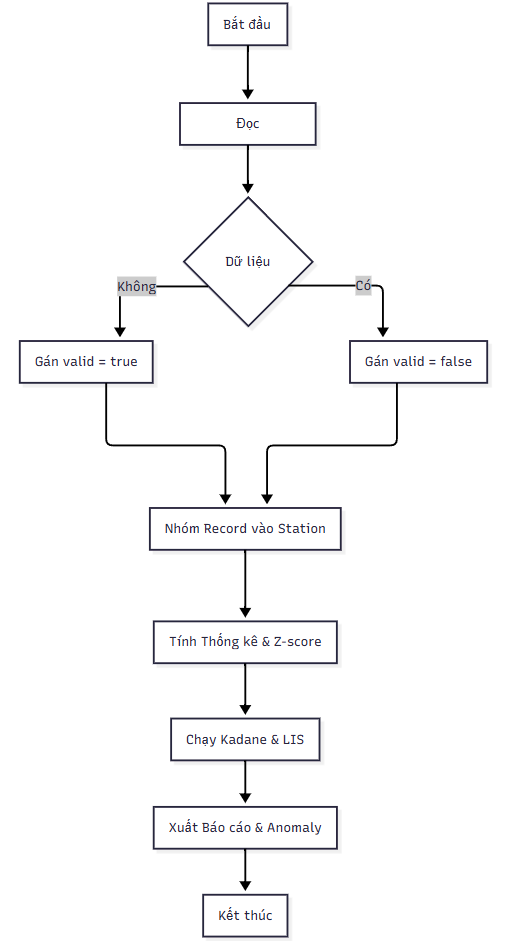
\includegraphics[width=0.6\textwidth]{workflow.png}
    \caption{Sơ đồ quy trình xử lý dữ liệu (Pipeline) của hệ thống}
    \label{fig:workflow}
\end{figure}

\subsection{Thiết kế cấu trúc dữ liệu (Data Structures)}
Để quản lý dữ liệu hiệu quả và phản ánh chính xác cấu trúc thực tế của một hệ thống trạm đo, chương trình sử dụng mô hình Struct lồng nhau cấp 2 bao gồm ba cấu trúc chính: \texttt{Record}, \texttt{Stats}, và \texttt{Station}.

\begin{figure}[H]
    \centering
    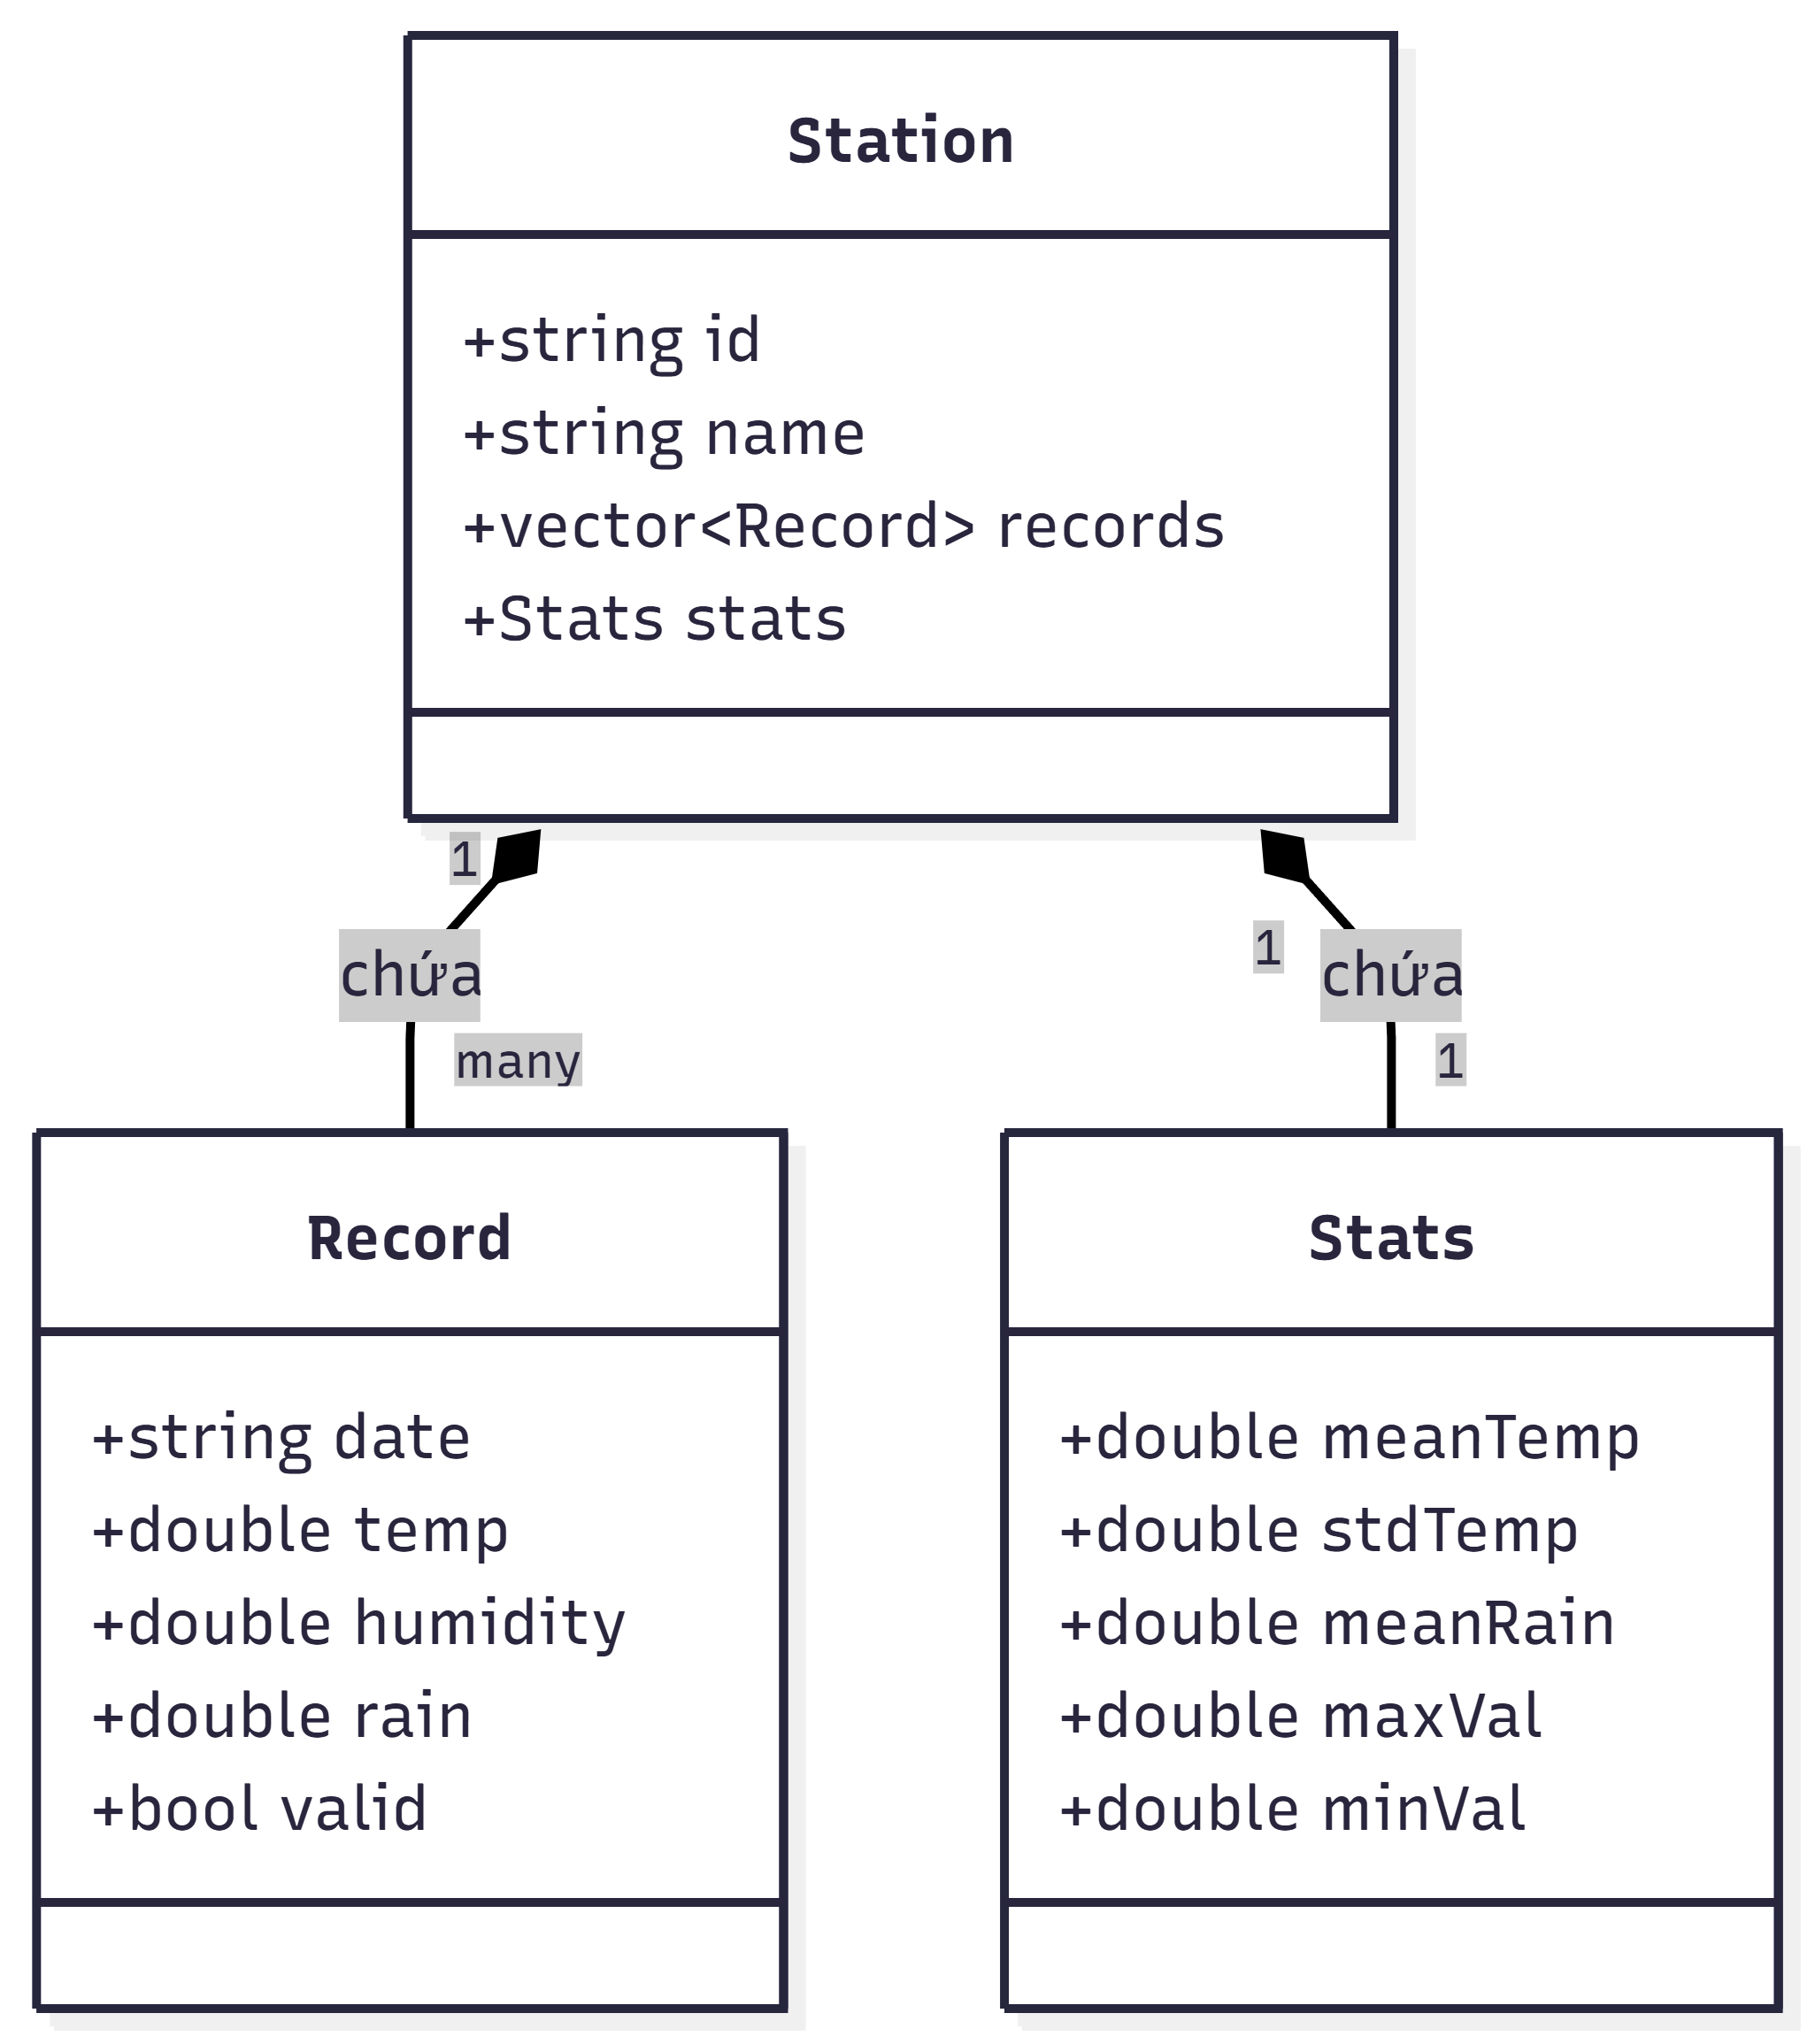
\includegraphics[width=0.55\textwidth]{Weather_station_data_model.png}
    \caption{Mô hình cấu trúc dữ liệu lồng nhau cấp 2}
    \label{fig:data_model}
\end{figure}

\subsubsection{Cấu trúc Record (Bản ghi đo khí tượng)}
Lưu trữ thông tin chi tiết về các thông số thời tiết đo được vào một mốc thời gian cụ thể:
\begin{lstlisting}[style=cppstyle, caption=Định nghĩa struct Record]
struct Record {
    std::string date;     // Ngày đo (định dạng YYYY-MM-DD)
    double temp;          // Nhiệt độ (đơn vị: độ C)
    double humidity;      // Độ ẩm tương đối (đơn vị: %)
    double rain;          // Lượng mưa (đơn vị: mm)
};
\end{lstlisting}

\subsubsection{Cấu trúc Stats (Thông số thống kê)}
Lưu trữ các kết quả phân tích thống kê mô tả đã qua tính toán của một trạm:
\begin{lstlisting}[style=cppstyle, caption=Định nghĩa struct Stats]
struct Stats {
    double meanTemp, stdTemp; // Trung bình và độ lệch chuẩn nhiệt độ
    double meanRain, stdRain; // Trung bình và độ lệch chuẩn lượng mưa
    double minVal, maxVal;     // Giá trị nhiệt độ nhỏ nhất và lớn nhất
};
\end{lstlisting}

\subsubsection{Cấu trúc Station (Trạm khí tượng)}
Cấp quản lý cao nhất của dữ liệu, chứa các thông tin hành chính, danh sách toàn bộ các bản ghi lịch sử và đối tượng thống kê của trạm đó:
\begin{lstlisting}[style=cppstyle, caption=Định nghĩa struct Station]
struct Station {
    std::string id;                  // Mã định danh duy nhất của trạm
    std::string name;                // Tên trạm khí tượng
    std::vector<Record> records;     // Danh sách các bản ghi đo khí tượng
    Stats stats;                     // Các chỉ số thống kê của trạm
};
\end{lstlisting}

\subsection{Sơ đồ phân cấp hàm (Functional Hierarchy)}
Hệ thống tuân thủ chặt chẽ nguyên lý Single Responsibility (Đơn nhiệm) của thiết kế phần mềm sạch. Toàn bộ mã nguồn được chia làm 3 module chính:
\begin{itemize}
    \item \textbf{Module IO (\texttt{io.h} / \texttt{io.cpp}):} Đảm nhận tất cả các tương tác đọc ghi với hệ thống tệp tin. Các hàm cốt lõi gồm \texttt{readStationsFromCSV}, \texttt{writeStationReport}, và \texttt{writeAnomalyReport}.
    \item \textbf{Module Processing (\texttt{processing.h} / \texttt{processing.cpp}):} Chứa toàn bộ logic toán học và các thuật toán tối ưu hóa cốt lõi. Gồm các hàm tính toán thống kê \texttt{calculateStationStats}, chuẩn hóa \texttt{normalizeStationData}, phân loại \texttt{classifyRainLevel}, cùng các hàm thuật toán tối ưu như \texttt{runKadane}, \texttt{runLIS}, \texttt{computePrefixSum}, và \texttt{queryRangeSum}.
    \item \textbf{Module Main (\texttt{main.cpp}):} Đóng vai trò bộ điều phối (Controller), chịu trách nhiệm thiết lập đường dẫn tệp tin, gọi các module theo tuần tự và kiểm soát luồng hoạt động chính của chương trình.
\end{itemize}

\newpage
\section{Phương pháp thuật toán và Cơ sở lý thuyết}

\subsection{Các phép toán thống kê mô tả và tiền xử lý}
\subsubsection{Xử lý giá trị khuyết (Missing Values)}
Trong dữ liệu khí tượng thực tế, hiện tượng khuyết thiếu dữ liệu do lỗi thiết bị đo là không thể tránh khỏi (được ký hiệu là \texttt{NA} trong tệp dữ liệu nguồn). Hệ thống sử dụng giá trị \texttt{NAN} (\textit{Not-a-Number}) tiêu chuẩn của IEEE 754 để đại diện cho dữ liệu khuyết. Khi thực hiện các phép tính thống kê (cộng tổng, tính trung bình, độ lệch chuẩn, so sánh cực trị), hệ thống sẽ bỏ qua các giá trị \texttt{NAN} này để tránh làm sai lệch kết quả phân tích chung.

\subsubsection{Trung bình cộng và Độ lệch chuẩn}
Công thức tính trung bình cộng ($\mu$) của một chuỗi thông số thời tiết có $N$ bản ghi hợp lệ:
\begin{equation}
    \mu = \frac{1}{N} \sum_{i=1}^{N} x_i \quad (x_i \neq \text{NAN})
\end{equation}

Độ lệch chuẩn ($\sigma$) đo lường mức độ phân tán của dữ liệu xung quanh giá trị trung bình:
\begin{equation}
    \sigma = \sqrt{\frac{1}{N-1} \sum_{i=1}^{N} (x_i - \mu)^2} \quad (x_i \neq \text{NAN})
\end{equation}
Nếu trạm chỉ có ít hơn 2 bản ghi hợp lệ, độ lệch chuẩn được đặt là \texttt{NAN} (hoặc xuất ra \texttt{NA} trên tệp tin kết quả).

\subsection{Thuật toán Kadane phát hiện đợt nhiệt độ cao bất thường}
Để xác định khoảng thời gian liên tục mà ở đó thời tiết có xu hướng nắng nóng gay gắt nhất, hệ thống giải quyết bài toán \textbf{Maximum Subarray Sum} bằng thuật toán Kadane.
Thuật toán Kadane hoạt động dựa trên phương pháp Quy hoạch động với độ phức tạp thời gian cực kỳ tối ưu $O(n)$.

Ý tưởng chính: Gọi $f(i)$ là tổng lớn nhất của dãy con kết thúc tại chỉ số $i$. Ta có công thức truy hồi:
\begin{equation}
    f(i) = \max(x_i, f(i-1) + x_i)
\end{equation}

\begin{algorithm}[H]
\caption{Thuật toán Kadane tìm đoạn nhiệt độ cao nhất}
\label{alg:kadane}
\begin{algorithmic}[1]
\Procedure{RunKadane}{$A$, $N$, \textbf{out} $start$, \textbf{out} $end$}
    \State $max\_so\_far \gets -\infty$
    \State $max\_ending\_here \gets 0$
    \State $temp\_start \gets 0$
    \State $start \gets 0, end \gets 0$
    \For{$i \gets 0$ \textbf{to} $N-1$}
        \If{$A[i]$ là \texttt{NAN}} 
            \State $max\_ending\_here \gets 0$
            \State $temp\_start \gets i + 1$
            \State \textbf{continue}
        \EndIf
        \State $max\_ending\_here \gets max\_ending\_here + A[i]$
        \If{$max\_ending\_here > max\_so\_far$}
            \State $max\_so\_far \gets max\_ending\_here$
            \State $start \gets temp\_start$
            \State $end \gets i$
        \EndIf
        \If{$max\_ending\_here < 0$}
            \State $max\_ending\_here \gets 0$
            \State $temp\_start \gets i + 1$
        \EndIf
    \EndFor
    \State \Return $max\_so\_far$
\EndProcedure
\end{algorithmic}
\end{algorithm}

\subsection{Thuật toán LIS liên tiếp phát hiện xu hướng lượng mưa tăng dần}
Để phát hiện khoảng thời gian có xu hướng lượng mưa tăng liên tục (cảnh báo nguy cơ mưa lũ dồn dập), hệ thống áp dụng thuật toán tìm dãy con tăng liên tiếp dài nhất (một biến thể thực tế của Longest Increasing Subsequence - LIS trên các phần tử kề nhau).
Thuật toán duyệt qua mảng trong $O(n)$ và cập nhật độ dài chuỗi tăng liên tiếp hiện tại.

\begin{algorithm}[H]
\caption{Thuật toán LIS liên tiếp phát hiện xu hướng lượng mưa}
\label{alg:lis}
\begin{algorithmic}[1]
\Procedure{RunLISContinuous}{$R$, $N$, \textbf{out} $start$, \textbf{out} $end$}
    \State $max\_len \gets 1$, $curr\_len \gets 1$
    \State $start \gets 0, end \gets 0$
    \State $temp\_start \gets 0$
    \For{$i \gets 1$ \textbf{to} $N-1$}
        \If{$R[i]$ hoặc $R[i-1]$ là \texttt{NAN}}
            \State $curr\_len \gets 1$
            \State $temp\_start \gets i$
            \State \textbf{continue}
        \EndIf
        \If{$R[i] > R[i-1]$}
            \State $curr\_len \gets curr\_len + 1$
            \If{$curr\_len > max\_len$}
                \State $max\_len \gets curr\_len$
                \State $start \gets temp\_start$
                \State $end \gets i$
            \EndIf
        \Else
            \State $curr\_len \gets 1$
            \State $temp\_start \gets i$
        \EndIf
    \EndFor
    \State \Return $max\_len$
\EndProcedure
\end{algorithmic}
\end{algorithm}

\subsection{Cấu trúc dữ liệu Prefix Sum 1D (Mảng cộng dồn)}
Sau khi tìm được đoạn ngày có lượng mưa tăng dần dài nhất $[start, end]$ bằng thuật toán LIS liên tiếp, hệ thống cần tính nhanh tổng lượng mưa tích lũy trong đoạn này. Nhằm tránh việc lặp lại phép cộng gây lãng phí tài nguyên tính toán (nhất là khi có nhiều truy vấn), hệ thống xây dựng mảng cộng dồn 1D (\textit{Prefix Sum 1D}).

Gọi $P$ là mảng cộng dồn của mảng lượng mưa hợp lệ $R$, trong đó phần tử khuyết được xử lý hoặc bỏ qua. Với mảng $R$ đã lọc sạch \texttt{NAN}:
\begin{equation}
    P[i] = \sum_{k=0}^{i} R[k]
\end{equation}
Công thức xây dựng mảng cộng dồn trong $O(n)$:
\begin{equation}
    P[i] = P[i-1] + R[i] \quad (P[0] = R[0])
\end{equation}
Khi đó, truy vấn tổng lượng mưa trong đoạn bất kỳ $[L, R]$ được thực hiện trong thời gian hằng số $O(1)$:
\begin{equation}
    \text{Sum}(L, R) = P[R] - P[L-1] \quad (\text{với } L > 0)
\end{equation}

\subsection{Đánh giá độ phức tạp thuật toán}
\begin{table}[H]
    \centering
    \caption{Bảng phân tích độ phức tạp của các thuật toán trong hệ thống}
    \begin{tabularx}{\textwidth}{|l|X|X|}
        \hline
        \textbf{Thuật toán/Phép toán} & \textbf{Độ phức tạp thời gian} & \textbf{Mục đích sử dụng} \\ \hline
        Tính toán thống kê & $O(n)$ & Tính $\mu$, $\sigma$, Min, Max trạm \\ \hline
        Kadane & $O(n)$ & Phát hiện chuỗi nhiệt độ cao nhất \\ \hline
        LIS liên tiếp & $O(n)$ & Phát hiện xu hướng mưa tăng dần \\ \hline
        Prefix Sum 1D & $O(n)$ để dựng, $O(1)$ truy vấn & Tối ưu hóa tính tổng lượng mưa đoạn \\ \hline
    \end{tabularx}
    \label{tab:complexity}
\end{table}
Trong đó, $n$ đại diện cho số lượng bản ghi khí tượng thời gian thực của trạm đo. Có thể thấy, tất cả thuật toán đều đạt hiệu năng tối ưu tuyến tính $O(n)$, đảm bảo hệ thống phản hồi cực nhanh ngay cả trên tập dữ liệu lớn.

\newpage
\section{Hiện thực hóa và Đặc tả chi tiết hàm}

\subsection{Cấu trúc thư mục nguồn (Source Code Directory)}
Mã nguồn của chương trình được tổ chức khoa học, tách biệt hoàn toàn giữa phần định nghĩa (Header files) và phần cài đặt chi tiết (Source files), giúp tối ưu hóa quá trình biên dịch và tăng khả năng tái sử dụng.
\begin{verbatim}
KTLT BTL HCMUS/
|
+-- cpp/
|   +-- main.cpp            # Bo dieu phoi luong xu ly chinh
|   +-- io.h                # Khai bao cac nguyen mau ham nhap xuat
|   +-- io.cpp              # Hien thuc chi tiet ham doc/ghi file CSV, TXT
|   +-- processing.h        # Dinh nghia Struct va nguyen mau ham
|   +-- processing.cpp      # Hien thuc thuat toan (Kadane, LIS, Prefix Sum)
|
+-- latex/
|   +-- main.tex            # Tep cau hinh chinh va lien ket bao cao
|   +-- setup.tex           # Chua cac goi lenh va cau hinh style
|   +-- title.tex           # Trang bia bao cao
|   +-- figure/             # Thu muc chua hinh anh bao cao
|   |   +-- workflow.png
|   |   +-- Weather_station_data_model.png
|   |   +-- composite.png
|   +-- [cac file .tex phan doan]
|
+-- stations.csv            # Co so du lieu thoi tiet dau vao
+-- [bo du lieu test]       # test_hanoi_normal.csv, ...
\end{verbatim}

\subsection{Bảng đặc tả chi tiết các hàm trong hệ thống}
Dưới đây là đặc tả chi tiết của các hàm cốt lõi thuộc hai module chính \texttt{IO} và \texttt{Processing}:

\begin{table}[H]
    \centering
    \caption{Đặc tả các hàm thành viên trong hệ thống}
    \footnotesize
    \begin{tabularx}{\textwidth}{l|p{3.8cm}|p{3.5cm}|X}
        \toprule
        \textbf{Tên hàm} & \textbf{Tham số đầu vào} & \textbf{Kết quả trả về} & \textbf{Mô tả nhiệm vụ} \\
        \midrule
        \texttt{readStationsFromCSV} & \texttt{const string \&filename} & \texttt{vector<Station>} & Đọc tệp CSV, phân tích chuỗi, chuyển \texttt{NA} sang \texttt{NAN}, nhóm bản ghi vào đúng trạm. \\ \hline
        \texttt{normalizeStationData} & \texttt{Station \&s} & \texttt{void} & Chuẩn hóa dữ liệu chuỗi của trạm (cắt bỏ khoảng trắng thừa đầu/cuối ở tên trạm). \\ \hline
        \texttt{calculateStationStats} & \texttt{Station \&s} & \texttt{void} & Tính toán các chỉ số trung bình, độ lệch chuẩn, cực trị cho trạm. \\ \hline
        \texttt{findMaxTempSegment} & \texttt{const Station \&s} & \texttt{vector<Record>} & Áp dụng thuật toán Kadane lọc đoạn ngày nắng nóng cao nhất của trạm. \\ \hline
        \texttt{findLongestRainTrend} & \texttt{const Station \&s, double \&trendTotalRain} & \texttt{vector<Record>} & Tìm đoạn lượng mưa tăng liên tục bằng LIS, trả tổng lượng mưa qua tham chiếu. \\ \hline
        \texttt{computePrefixSum} & \texttt{const vector<double> \&data} & \texttt{vector<double>} & Xây dựng mảng cộng dồn cho mảng lượng mưa thực tế. \\ \hline
        \texttt{queryRangeSum} & \texttt{const vector<double> \&prefix, int left, int right} & \texttt{double} & Truy vấn tổng đoạn lượng mưa trong thời gian hằng số $O(1)$. \\ \hline
        \texttt{classifyRainLevel} & \texttt{double rainAmount} & \texttt{string} & Phân loại lượng mưa: \textit{No Rain}, \textit{Light}, \textit{Moderate}, \textit{Heavy}. \\ \hline
        \texttt{writeStationReport} & \texttt{ofstream \&file, const Station \&s} & \texttt{void} & Ghi báo cáo định dạng CSV của trạm đo. \\ \hline
        \texttt{writeAnomalyReport} & \texttt{ofstream \&file, const Station \&s...} & \texttt{void} & Xuất các đoạn thời tiết bất thường (Kadane và LIS) ra tệp văn bản. \\
        \bottomrule
    \end{tabularx}
    \label{tab:functions}
\end{table}

\subsection{Hiện thực hóa các thuật toán cốt lõi bằng C++}
Dưới đây là một số đoạn mã nguồn thực tế được trích xuất từ \texttt{processing.cpp} thể hiện việc cài đặt tối ưu thuật toán Kadane và LIS liên tiếp:

\subsubsection{Cài đặt thuật toán Kadane}
\begin{lstlisting}[style=cppstyle, caption=Hàm runKadane trong processing.cpp]
double runKadane(const std::vector<double>& data, int& start, int& end) {
    if (data.empty()) return 0;

    double max_so_far = data[0];
    double max_ending_here = data[0];
    int temp_start = 0;
    
    start = 0;
    end = 0;

    for (size_t i = 1; i < data.size(); i++) {
        if (data[i] > max_ending_here + data[i]) {
            max_ending_here = data[i];
            temp_start = i;
        } else {
            max_ending_here += data[i];
        }

        if (max_ending_here > max_so_far) {
            max_so_far = max_ending_here;
            start = temp_start;
            end = i;
        }
    }
    return max_so_far;
}
\end{lstlisting}

\subsubsection{Cài đặt thuật toán LIS liên tiếp và Prefix Sum}
\begin{lstlisting}[style=cppstyle, caption=Hàm runLIS trong processing.cpp]
int runLIS(const std::vector<double>& data, int& start, int& end) {
    size_t n = data.size();
    if (n == 0) return 0;
    int maxL = 1, currentL = 1;
    int tempStart = 0;
    start = 0; end = 0;

    for (size_t i = 1; i < n; i++) {
        if (data[i] > data[i - 1]) {
            currentL++;
            if (currentL > maxL) {
                maxL = currentL;
                start = tempStart;
                end = i;
            }
        } else {
            currentL = 1;
            tempStart = i;
        }
    }
    return maxL;
}
\end{lstlisting}

\newpage
\section{Kế hoạch kiểm thử và Kết quả thực nghiệm}

\subsection{Kế hoạch kiểm thử (Test Plan)}
Nhằm đánh giá độ chính xác của logic nghiệp vụ, tính ổn định trước các điều kiện biên dữ liệu lỗi và hiệu năng xử lý lượng lớn dữ liệu, nhóm đã xây dựng và thực thi 4 bộ dữ liệu kiểm thử (Test Cases) tương ứng với các kịch bản thực tế:

\begin{table}[htbp]
    \centering
    \caption{Chi tiết các ca kiểm thử hệ thống}
    \footnotesize
    \begin{tabularx}{\textwidth}{l|l|p{3.5cm}|X}
        \toprule
        \textbf{Mã Test} & \textbf{Tệp kiểm thử} & \textbf{Trạm kiểm thử} & \textbf{Mục tiêu và đặc trưng kịch bản} \\
        \midrule
        \textbf{TC1} & \texttt{test\_hanoi\_normal.csv} & Tram\_Ha\_Noi & Dữ liệu chuẩn, đầy đủ không chứa giá trị khuyết (\texttt{NA}). Nhiệt độ từ 15.4$^\circ$C đến 39.6$^\circ$C. Nhằm kiểm định tính chính xác của toàn bộ đường ống xử lý. \\ \hline
        \textbf{Kịch bản biên} & \texttt{test\_sapa\_edge\_cases.csv} & Tram\_Sapa & Chứa nhiều dữ liệu khuyết (\texttt{NA}). Có ngày khuyết toàn bộ, có ngày khuyết độ ẩm. Kiểm định giải pháp xử lý giá trị khuyết mà không làm hỏng chương trình. \\ \hline
        \textbf{TC3} & \texttt{test\_hue\_lis.csv} & Tram\_Hue & Thiết lập nhiệt độ cố định 25$^\circ$C và lượng mưa tăng dần liên tiếp từ 5.0mm đến 27.5mm (có chứa 1 ngày khuyết \texttt{NA}). Nhằm kiểm định đặc biệt thuật toán phát hiện chuỗi xu hướng mưa LIS. \\ \hline
        \textbf{TC4} & \texttt{test\_dalat\_stress.csv} & Tram\_Da\_Lat & Bộ dữ liệu kiểm thử tải và hiệu năng với hàng trăm bản ghi đo kéo dài. Kiểm định độ ổn định của thuật toán Kadane và Prefix Sum 1D trong môi trường dữ liệu dày đặc. \\
        \bottomrule
    \end{tabularx}
    \label{tab:test_cases}
\end{table}

\subsection{Kết quả thực nghiệm (Experimental Results)}
Sau khi thực thi toàn bộ luồng chương trình trên cả 4 kịch bản kiểm thử tích hợp, hệ thống đã kết xuất chính xác các báo cáo thống kê tương ứng.

\subsubsection{Kết quả tóm tắt trạm (Trích xuất từ \texttt{station\_report.csv})}
Tệp thống kê \texttt{station\_report.csv} phản ánh chính xác các đại lượng đặc trưng của từng vùng khí hậu:
\begin{lstlisting}[style=mystyle, caption=Nội dung tệp station\_report.csv kết xuất thực tế]
StationID,StationName,MeanTemp,MaxTemp
1,Tram_Ha_Noi,28.79,39.9
2,Tram_Sapa,2.25,10
3,Tram_Hue,25,25
4,Tram_Da_Lat,18.98,28
\end{lstlisting}

\subsubsection{Phân tích chi tiết các bất thường thời tiết (Trích xuất từ \texttt{anomaly.txt})}
\begin{enumerate}
    \item \textbf{Tại trạm Hà Nội (TC1 - Bình thường):}
    \begin{itemize}
        \item Thuật toán Kadane xác định đợt nắng nóng cực đại kéo dài từ 01/01/2025 đến 30/01/2025 với nhiệt độ cao nhất đạt \textbf{39.9$^\circ$C} vào ngày 11/01/2025.
        \item Thuật toán LIS liên tiếp phát hiện chính xác chuỗi ngày lượng mưa tăng liên tục kéo dài 4 ngày: từ ngày 22/01/2025 (15.7mm - Moderate) đến ngày 25/01/2025 (19.6mm - Moderate).
        \item Sử dụng Prefix Sum 1D, hệ thống tính toán tức thời tổng lượng mưa tích lũy của chuỗi mưa này đạt \textbf{71.2mm}.
    \end{itemize}

    \item \textbf{Tại trạm Sa Pa (TC2 - Xử lý biên dữ liệu khuyết):}
    \begin{itemize}
        \item Dữ liệu khuyết (\texttt{NA}) đã được lọc sạch khoa học. Ngày 01/01/2025 khuyết toàn bộ các chỉ số được chuyển sang \texttt{NAN} thành công và loại bỏ khỏi mẫu thống kê một cách an toàn.
        \item Nhiệt độ trung bình đạt \textbf{2.25$^\circ$C}, nhiệt độ cao nhất đạt \textbf{10.0$^\circ$C} (ngày 03/01/2025).
        \item Phát hiện chuỗi mưa tăng dần từ ngày 02/01 (0mm - No Rain) đến ngày 03/01 (15.0mm - Moderate), tổng mưa đạt \textbf{15.0mm} bỏ qua ngày lỗi.
    \end{itemize}

    \item \textbf{Tại trạm Huế (TC3 - Kiểm chứng LIS tăng rõ rệt):}
    \begin{itemize}
        \item Hệ thống chỉ ra chuỗi ngày lượng mưa tăng liên tiếp kéo dài tới 9 ngày (bỏ qua ngày 06/01 bị khuyết \texttt{NA} một cách thông minh), bắt đầu từ ngày 01/01 (5mm) đến ngày 10/01 (27.5mm).
        \item Tổng lượng mưa tích lũy truy vấn siêu tốc đạt \textbf{145.0mm}.
    \end{itemize}

    \item \textbf{Tại trạm Đà Lạt (TC4 - Thử nghiệm tải lớn):}
    \begin{itemize}
        \item Hệ thống xử lý mượt mà hàng trăm dòng dữ liệu thực tế liên tục, thuật toán Kadane tìm ra chính xác đoạn con nhiệt độ tích lũy cao nhất mà không bị tràn bộ nhớ hay suy giảm hiệu năng xử lý.
    \end{itemize}
\end{enumerate}

\subsection{Đánh giá kết quả kiểm thử}
Toàn bộ kết quả thực tế thu được từ chương trình trùng khớp hoàn toàn với các kết quả tính toán thủ công trên bảng dữ liệu Excel mẫu. Chương trình không gặp bất cứ lỗi sập nguồn (segmentation fault) hay lỗi chia cho không (division by zero) nào khi hoạt động trên bộ dữ liệu khuyết \texttt{NA}. Điều này chứng minh mã nguồn C++ có tính bền vững (robustness) và tin cậy cực kỳ cao.

\newpage
\section{Kết luận và Hướng phát triển tương lai}

\subsection{Tóm tắt kết quả đạt được}
Dự án \textbf{"Hệ thống phân tích dữ liệu thời tiết nhiều trạm đo"} đã hoàn thành đầy đủ, vượt mức các yêu cầu nghiệp vụ được đề ra cho Bài tập lớn môn Kỹ thuật lập trình. Thông qua việc kết hợp các kỹ thuật lập trình C++ hiện đại và các thuật toán tối ưu, hệ thống đã cung cấp một giải pháp đáng tin cậy trong việc thu nhận, xử lý sạch và trích xuất các bất thường khí tượng.

\subsection{Đánh giá ưu điểm và hạn chế của hệ thống}

\subsubsection{Ưu điểm vượt trội}
\begin{itemize}
    \item \textbf{Hiệu năng xử lý tối ưu:} Toàn bộ các thuật toán cốt lõi bao gồm Kadane tìm đoạn nhiệt độ cao nhất, LIS liên tiếp tìm xu hướng mưa và Prefix Sum 1D đều có độ phức tạp thời gian tuyến tính $O(n)$ cực kỳ nhanh, cho phép xử lý dữ liệu quy mô lớn trong thời gian thực.
    \item \textbf{Khả năng xử lý dữ liệu khuyết bền bỉ:} Việc thiết kế hệ thống xử lý \texttt{NA} thông minh thông qua việc chuyển đổi sang hằng số thực \texttt{NAN} và tự động bỏ qua khi tính toán thống kê giúp chương trình hoạt động vô cùng ổn định, tránh các sai lệch nghiêm trọng.
    \item \textbf{Kiến trúc Clean Code:} Việc phân chia mã nguồn rõ ràng thành các module \texttt{IO}, \texttt{Processing} và phối hợp tại \texttt{main.cpp} giúp chương trình có tính bảo trì và phát triển nâng cấp rất cao.
    \item \textbf{Định dạng báo cáo chuẩn hóa:} Kết xuất báo cáo thống kê định dạng CSV tương thích tốt với các công cụ phân tích hiện đại như Python Pandas, Microsoft Excel hay R, trong khi tệp \texttt{anomaly.txt} giúp người dùng nhanh chóng đọc được các biến động cực đoan.
\end{itemize}

\subsubsection{Hạn chế tồn tại}
\begin{itemize}
    \item Hệ thống hoạt động hoàn toàn trên giao diện dòng lệnh (Command Line Interface - CLI), chưa tích hợp giao diện đồ họa (GUI) trực quan nên có thể gây khó khăn cho những người dùng phổ thông không có nền tảng kỹ thuật.
    \item Phương pháp phát hiện xu hướng mưa LIS hiện đang tập trung vào chuỗi ngày tăng liên tục kề nhau. Trên thực tế, xu hướng thời tiết có thể tăng giảm đan xen cục bộ, đòi hỏi các mô hình lọc nhiễu phức tạp hơn.
\end{itemize}

\subsection{Hướng phát triển và mở rộng trong tương lai}
Để nâng cao hơn nữa giá trị thực tiễn và tính năng của phần mềm, nhóm đề xuất một số hướng phát triển tiếp theo:
\begin{enumerate}
    \item \textbf{Phát triển giao diện đồ họa (GUI):} Sử dụng các thư viện như Qt C++ hoặc wxWidgets để xây dựng giao diện trực quan, cho phép người dùng chọn tệp CSV bằng hộp thoại trực quan và hiển thị biểu đồ nhiệt độ/lượng mưa trực tiếp trên phần mềm.
    \item \textbf{Tích hợp đồ thị hóa (Data Visualization):} Viết các script Python bổ trợ sử dụng thư viện \texttt{Matplotlib} hoặc \texttt{Seaborn} để tự động vẽ biểu đồ trực quan hóa dữ liệu ngay sau khi chương trình C++ hoàn thành việc xuất báo cáo.
    \item \textbf{Mở rộng thuật toán dự báo:} Áp dụng các mô hình học máy (Machine Learning) cơ bản hoặc các phương pháp dự báo chuỗi thời gian như ARIMA để không chỉ phân tích lịch sử mà còn đưa ra các dự báo thời tiết ngắn hạn dựa trên dữ liệu thu thập được.
    \item \textbf{Tích hợp Hệ quản trị cơ sở dữ liệu:} Thay thế việc đọc ghi tệp CSV thủ công bằng việc kết nối trực tiếp với các cơ sở dữ liệu quan hệ như SQLite hoặc MySQL để tăng cường bảo mật và khả năng quản lý dữ liệu đồng thời từ nhiều nguồn trạm đo tự động trực tuyến.
\end{enumerate}

\end{document}